% DYSLEXIA SWITCH
\newif\ifdys
		
				% ENABLE or DISABLE font change
				% use XeLaTeX if true
				\dystrue
				\dysfalse


\ifdys

\documentclass[a4paper, 14pt]{extarticle}
\usepackage{amsmath,amsfonts,amsthm,amssymb,mathtools}

\tracinglostchars=3 % Report an error if a font does not have a symbol.
\usepackage{fontspec}
\usepackage{unicode-math}
\defaultfontfeatures{ Ligatures=TeX,
                      Scale=MatchUppercase }

\setmainfont{OpenDyslexic}[Scale=1.0]
\setmathfont{Fira Math} % Or maybe try KPMath-Sans?
\setmathfont{OpenDyslexic Italic}[range=it/{Latin,latin}]
\setmathfont{OpenDyslexic}[range=up/{Latin,latin,num}]

\else

\documentclass[a4paper, 12pt]{extarticle}

\usepackage[utf8x]{inputenc}
%fonts
\usepackage{amsmath,amsfonts,amsthm,amssymb,mathtools}
% comment below to default to computer modern
\usepackage{libertinus,libertinust1math}

\fi


\usepackage[french]{babel}
\usepackage[
a4paper,
margin=2cm,
nomarginpar,% We don't want any margin paragraphs
]{geometry}
\usepackage{icomma}

\usepackage{fancyhdr}
\usepackage{array}
\usepackage{hyperref}

\usepackage{multicol, enumerate}
\newcolumntype{P}[1]{>{\centering\arraybackslash}p{#1}}


\usepackage{stackengine}
\newcommand\xrowht[2][0]{\addstackgap[.5\dimexpr#2\relax]{\vphantom{#1}}}

% theorems

\theoremstyle{plain}
\newtheorem{theorem}{Th\'eor\`eme}
\newtheorem*{sol}{Solution}
\theoremstyle{definition}
\newtheorem{ex}{Exercice}
\newtheorem*{rpl}{Rappel}
\newtheorem{enigme}{Énigme}

% corps
\usepackage{calrsfs}
\newcommand{\C}{\mathcal{C}}
\newcommand{\R}{\mathbb{R}}
\newcommand{\Rnn}{\mathbb{R}^{2n}}
\newcommand{\Z}{\mathbb{Z}}
\newcommand{\N}{\mathbb{N}}
\newcommand{\Q}{\mathbb{Q}}

% variance
\newcommand{\Var}[1]{\text{Var}(#1)}

% domain
\newcommand{\D}{\mathcal{D}}


% date
\usepackage{advdate}
\AdvanceDate[0]


% plots
\usepackage{pgfplots}

% table line break
\usepackage{makecell}
%tablestuff
\def\arraystretch{2}
\setlength\tabcolsep{15pt}

%subfigures
\usepackage{subcaption}

\definecolor{myg}{RGB}{56, 140, 70}
\definecolor{myb}{RGB}{45, 111, 177}
\definecolor{myr}{RGB}{199, 68, 64}

% fake sections with no title to move around the merged pdf
\newcommand{\fakesection}[1]{%
  \par\refstepcounter{section}% Increase section counter
  \sectionmark{#1}% Add section mark (header)
  \addcontentsline{toc}{section}{\protect\numberline{\thesection}#1}% Add section to ToC
  % Add more content here, if needed.
}


% SOLUTION SWITCH
\newif\ifsolutions
				\solutionstrue
				%\solutionsfalse

\ifsolutions
	\newcommand{\exe}[2]{
		\begin{ex} #1  \end{ex}
		\begin{sol} #2 \end{sol}
	}
\else
	\newcommand{\exe}[2]{
		\begin{ex} #1  \end{ex}
	}
	
\fi


% tableaux var, signe
\usepackage{tkz-tab}


%pinfty minfty
\newcommand{\pinfty}{{+}\infty}
\newcommand{\minfty}{{-}\infty}

\begin{document}


\usepackage{minted}

\SetDate[17/10/2025]

\begin{document}
\pagestyle{fancy}
\fancyhead[L]{Seconde}
\fancyhead[C]{\textbf{Représenter des points dans le plan en Python}}
\fancyhead[R]{\today}

Le but de ce document est d'automatiser l'exercice \ref{exe:milieu-segment} de la feuille « Plan cartésien » à l'aide du langage de programmation Python.
Automatiser permet d'accélérer la vitesse de calcul.

\setcounter{Exercise}{9}
\exe{}{
	Représenter les points $A(1;1)$ et $B(3;-1)$ dans un repère orthonormé.
	Représenter le point
		\[ \lambda A + (1-\lambda)B, \]
	pour certaines valeurs de $\lambda$ (lu « lambda ») entre 0 et 1.
}{exe:milieu-segment}{}


\setlength\columnsep{30pt}

\subsection*{Stocker et afficher un nombre}

\begin{multicols}{2}
	\begin{itemize}
		\item
	Lorsqu'on écrit \texttt{x=0.5}, la valeur à droite du signe « = » est stockée dans la variable à gauche.
		\item
	La fonction \texttt{print(x)} permet d'afficher la valeur de la variable \texttt{x}.
	\end{itemize}
	
	\columnbreak
	\centering
	\begin{minipage}{.1\textwidth}
	\python{print}
	\end{minipage}
\end{multicols}

\begin{enumerate}[label=\warning]
	\item
	Il faut utiliser le point à la place de la virgule pour séparer la partie décimale de la partie entière des nombres.

	\item
	 Le signe « = » a un sens différent qu'en mathématiques. Il sert uniquement à stocker la valeur de droite dans la variable de gauche.

	\item
	 Certains noms de variables sont illégaux car déjà empruntés. Ils s'afficheront en couleur si c'est le cas (\texttt{lambda}, \texttt{for}, \texttt{while}, \dots).
\end{enumerate}

\subsection*{Multiplication et addition}

\begin{multicols}{2}
	\begin{enumerate}
		\item[+] : addition
		\item[-] : soustraction
		\item[*] : multiplication
		\item[/] : division
	\end{enumerate}
	
	L'usage des parenthèses et l'ordre des opérations sont identiques à ceux en mathématiques.
		
	\columnbreak
	\centering
	\begin{minipage}{.1\textwidth}
	\python{operations}
	\end{minipage}
\end{multicols}

\subsection*{Définir et stocker une liste de nombres}

\begin{multicols}{2}
	Une liste de nombres est créée avec des crochets. Les éléments sont séparés par des virgules.

	%Le signe « = » stocke la liste à droite dans la variable à gauche.
	\columnbreak
	\centering
	\begin{minipage}{.2\textwidth}
	\python{list}
	\end{minipage}
\end{multicols}

\subsection*{Parcourir une liste}

\begin{multicols}{2}
	Pour parcourir une liste, on utilise la boucle \texttt{for <variable> in <liste>}.
	Pour chaque élément de la liste, l'élément est stocké dans la variable, et tout le bloc est executé.
	
	\columnbreak
	\centering
	\begin{minipage}{.3\textwidth}
	\python{boucle}
	\end{minipage}
\end{multicols}

L'\textbf{indentation} (décalage par ajout d'espaces vides) est importante en Python car elle définit quelles lignes appartiennent ou non au bloc executé à chaque itération de la boucle.
On utilise la touche de tabulation \textbf{Tab} à gauche du clavier pour ajouter ces espaces vides (ou on appuie 4 fois sur la touche espace).

\newpage

\subsection*{Exemples}

\def\arraystretch{1}
\setlength\tabcolsep{5pt}
\begin{figure}[h]
\begin{subfigure}{.22\textwidth}
	\begin{tabular}{|c|c|c|c|}\hline
		Ligne & \texttt{a} & \texttt{b} & \texttt{m} \\ \hline
		$1$ &&& \\ \hline
		$2$ &&& \\ \hline
		$3$ &&& \\ \hline
		$4$ &&& \\ \hline
		$5$ &&& \\ \hline
		$6$ &&& \\ \hline
		$7$ &&& \\ \hline
		$8$ &&& \\ \hline
	\end{tabular}
\end{subfigure}
\begin{subfigure}{.24\textwidth}
\vspace{14pt}
\python{exemple1}
\end{subfigure}
\hspace{10pt}
\begin{subfigure}{.26\textwidth}
	\begin{tabular}{|c|c|c|c|}\hline
		Ligne & \texttt{a} & \texttt{b} & \texttt{temp} \\ \hline
		$1$ &&& \\ \hline
		$2$ &&& \\ \hline
		$3$ &&& \\ \hline
		$4$ &&& \\ \hline
		$5$ &&& \\ \hline
		$6$ &&& \\ \hline
		$7$ &&& \\ \hline
		$8$ &&& \\ \hline
	\end{tabular}
\end{subfigure}
%\hfill
\begin{subfigure}{.24\textwidth}
\vspace{15pt}
\python{exemple2}
\end{subfigure}

%\begin{subfigure}{.5\textwidth}
%\vspace{15pt}
%\python{exemple3}
%\end{subfigure}
%\hfill
%\begin{subfigure}{.45\textwidth}
%	\begin{tabular}{|c|c|c|}\hline
%		Ligne & \texttt{a} & \texttt{b} \\ \hline
%		$1$ && \\ \hline
%		$2$ && \\ \hline
%		$3$ && \\ \hline
%		$4$ && \\ \hline
%		$5$ && \\ \hline
%		$6$ && \\ \hline
%		$7$ && \\ \hline
%		$8$ && \\ \hline
%	\end{tabular}
%\end{subfigure}
\end{figure}


\subsection*{Représentation dans un repère}

La librairie \texttt{matplotlib} est utile pour placer des points dans un repère.

\begin{multicols}{2}
	La première ligne importe la librairie et la nomme \texttt{plt}.
	La deuxième ligne ajoute le point $(3 ; 4)$.
	La troisième ligne affiche le repère dans une nouvelle fenêtre.
	
	\columnbreak
	\centering
	\begin{minipage}{.3\textwidth}
	\python{scatter}
	\end{minipage}
\end{multicols}

\subsection*{Améliorations et expérimentations possibles}

Quelques améliorations possibles sont proposées avec des exemples d'implémentation hors contexte.
\begin{multicols}{2}
	\begin{itemize}[itemsep=9pt]
		\item Prendre une centaine de valeurs de $\lambda$ entre 0 et 1.
		\item Changer la couleur du point en fonction de la valeur de $\lambda$.
		\item Ajouter un quadrillage au repère.
		\item Centrer les axes des abscisses et des ordonnées.
		\item Ajuster la fenêtre en définissant les plages des abscisses et des ordonnées affichées.
		\item Que se passe-t-il si on prend des valeurs de $\lambda$ non comprises entre 0 et 1 ?
		\item Définir les variables $xM$ et $yM$ et implémenter le cacul de $\lambda$ en abscisse et en ordonnée vérifiant les équations
			\begin{align*}
				\lambda x_A + (1-\lambda) x_B = x_M, && \et && \lambda y_A + (1-\lambda) y_B = y_M.
			\end{align*}
		Imprimer les deux poids pour décider si $(2 ; 0), (1 ; 1), ( 1,5 ; 0,5), (2,5 ; -0,5)$ appartiennent à $[AB]$.
	\end{itemize}
	\vfill\null
	
	\columnbreak
	\centering
	\begin{minipage}{.3\textwidth}
	\python{ameliorations}
	\end{minipage}
\end{multicols}

%%%%%%%%%%%

\newpage
\fancyhead[C]{\textbf{Solutions}}

\subsection*{Exemples}

\def\arraystretch{1}
\setlength\tabcolsep{5pt}
\begin{figure}[h]
\begin{subfigure}{.245\textwidth}
	\begin{tabular}{|c|c|c|c|}\hline
		Ligne & \texttt{a} & \texttt{b} & \texttt{m} \\ \hline
		$1$ &5&& \\ \hline
		$2$ &5&15& \\ \hline
		$3$ &5&15&10.0 \\ \hline
		$4$ &5&15&10.0 \\ \hline
		$5$ &5&15&10.0 \\ \hline
		$6$ &15&15&10.0 \\ \hline
		$7$ &15&15&10.0 \\ \hline
		$8$ &15&15&10.0 \\ \hline
	\end{tabular}
\end{subfigure}
\begin{subfigure}{.24\textwidth}
\vspace{14pt}
\python{exemple1}
\end{subfigure}
%\hspace{5pt}
\begin{subfigure}{.26\textwidth}
	\begin{tabular}{|c|c|c|c|}\hline
		Ligne & \texttt{a} & \texttt{b} & \texttt{temp} \\ \hline
		$1$ &-4&& \\ \hline
		$2$ &-4&12& \\ \hline
		$3$ &-4&12& \\ \hline
		$4$ &-4&12& \\ \hline
		$5$ &-4&12&-4 \\ \hline
		$6$ &12&12&-4 \\ \hline
		$7$ &12&-4&-4 \\ \hline
		$8$ &12&-4&-4 \\ \hline
	\end{tabular}
\end{subfigure}
\begin{subfigure}{.24\textwidth}
\vspace{15pt}
\python{exemple2}
\end{subfigure}
\end{figure}

\subsection*{Améliorations et expérimentations possibles}

\setlength\columnsep{-100pt}
\begin{multicols}{2}
	\python{segment}
	
	\columnbreak
	\centering
	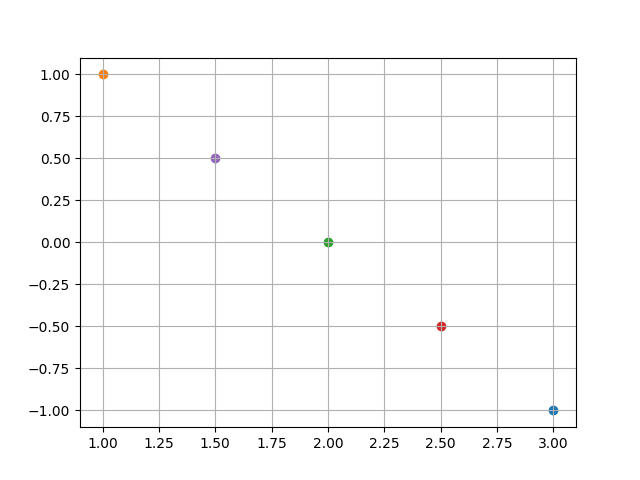
\includegraphics[scale=.7]{segment.png}
\end{multicols}
\newpage
\begin{multicols}{2}
	\python{segment-ameliore}
	\columnbreak
	\centering
	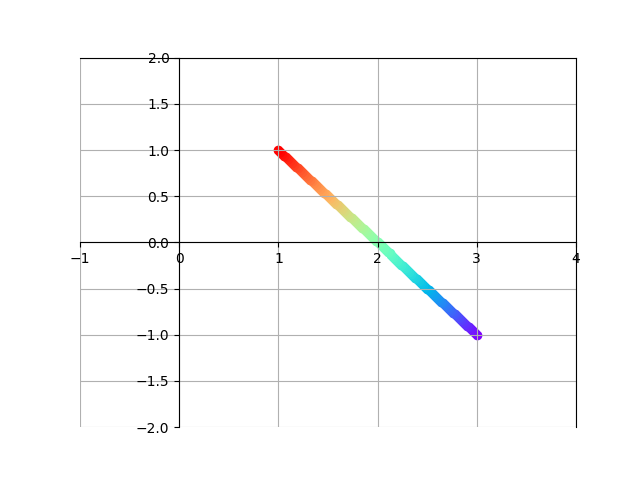
\includegraphics[scale=.7]{segment-ameliore.png}
\end{multicols}

\end{document}
